\documentclass[11pt, a4paper]{article}

\usepackage[affil-it]{authblk}
\usepackage{etoolbox}
\usepackage{lmodern}
\usepackage{titlesec}
\usepackage{float}
\usepackage{amsfonts}
\usepackage{hyperref}
\usepackage{listings}
\usepackage{color}
\usepackage{graphicx}
\usepackage{subcaption}
\usepackage{amsmath}
\usepackage{relsize}

\makeatletter
\patchcmd{\@maketitle}{\LARGE \@title}{\fontsize{20}{19.2}\selectfont\@title}{}{}
\makeatother

\renewcommand\Authfont{\fontsize{16}{14.4}\selectfont}
\renewcommand\Affilfont{\fontsize{12}{10.8}\itshape}

\title{\textbf{AE 706: Assignment 3}}
\author{Pavan R Hebbar - 130010046}

\definecolor{codegreen}{rgb}{0,0.6,0}
\definecolor{codegray}{rgb}{0.5,0.5,0.5}
\definecolor{codepurple}{rgb}{0.58,0,0.82}
\definecolor{backcolour}{rgb}{0.95,0.95,0.92}
 
\lstdefinestyle{mystyle}{
    backgroundcolor=\color{backcolour},   
    commentstyle=\color{codegreen},
    keywordstyle=\color{magenta},
    numberstyle=\tiny\color{codegray},
    stringstyle=\color{codepurple},
    basicstyle=\footnotesize,
    breakatwhitespace=false,         
    breaklines=true,                 
    captionpos=b,                    
    keepspaces=true,                 
    numbers=left,                    
    numbersep=5pt,                  
    showspaces=false,                
    showstringspaces=false,
    showtabs=false,                  
    tabsize=2
}
\lstset{style=mystyle}

\begin{document}
\maketitle
\newpage
\tableofcontents
\newpage
\section{Introduction:}
In this assignement we implement numerical schemes to solve the linear advection equation and analyse their stability

\section{Question 1:}
In this question we solve the given intial condition and boundary conditions using FTBS, FTFS and FTCS schemes with CFL values
0.8, 1.0 and 1.2.

\subsection{FTBS}
\subsubsection{CFL = 0.8}
\begin{figure}[H]
 \centering
 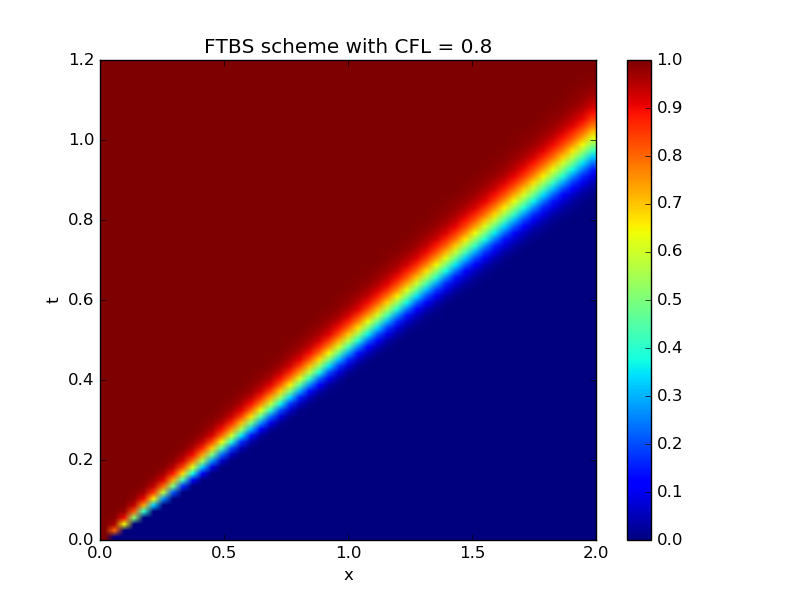
\includegraphics[width = 0.8\textwidth]{FTBS1_08.png}
 \caption{Color represents the magnitude of u at the given x and t}
\end{figure}

\begin{figure}[H]
 \centering
 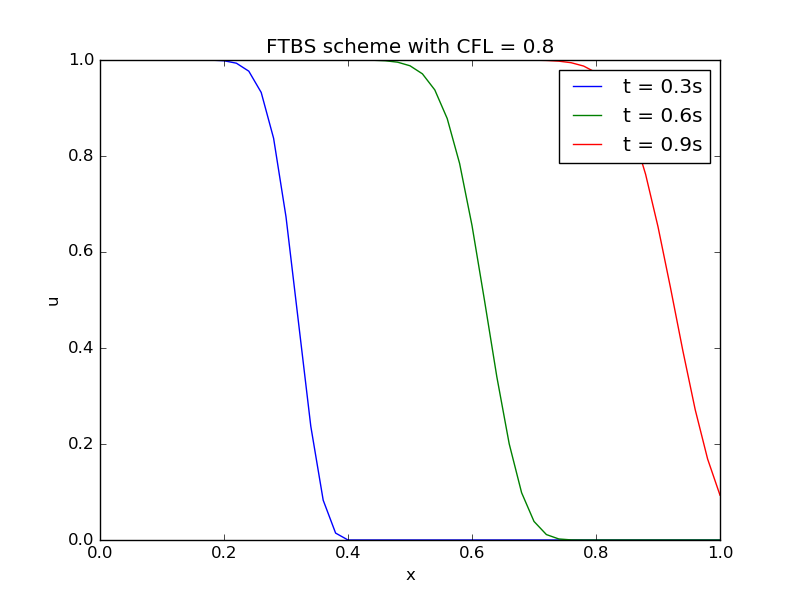
\includegraphics[width = 0.8\textwidth]{FTBS1_08_1.png}
 \caption{Plot of u v/s x for various t}
\end{figure}

We see that that the step function starts smoothening. This is because the higher frequency components dampen faster in
in comparison to lower frequencies.

\subsubsection{CFL = 1.0}
\begin{figure}[H]
 \centering
 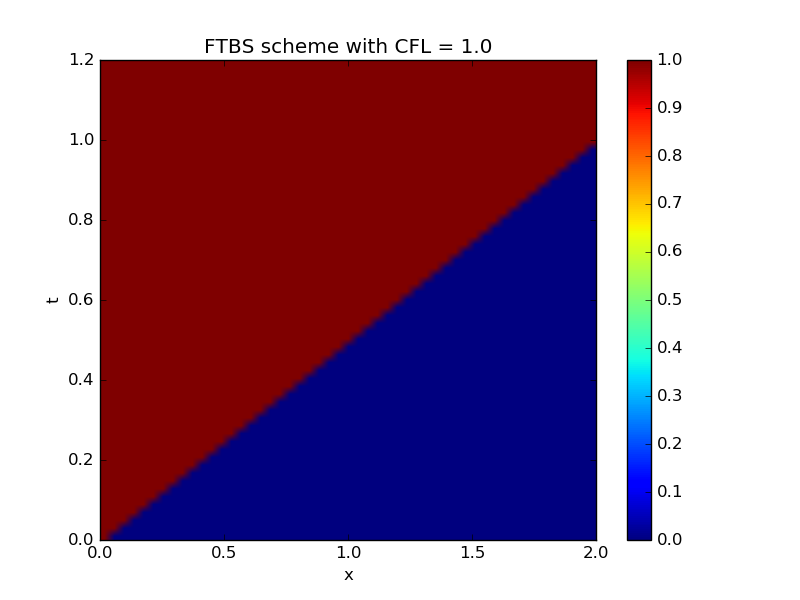
\includegraphics[width = 0.8\textwidth]{FTBS1_1.png}
 \caption{Color represents the magnitude of u at the given x and t}
\end{figure}

\begin{figure}[H]
 \centering
 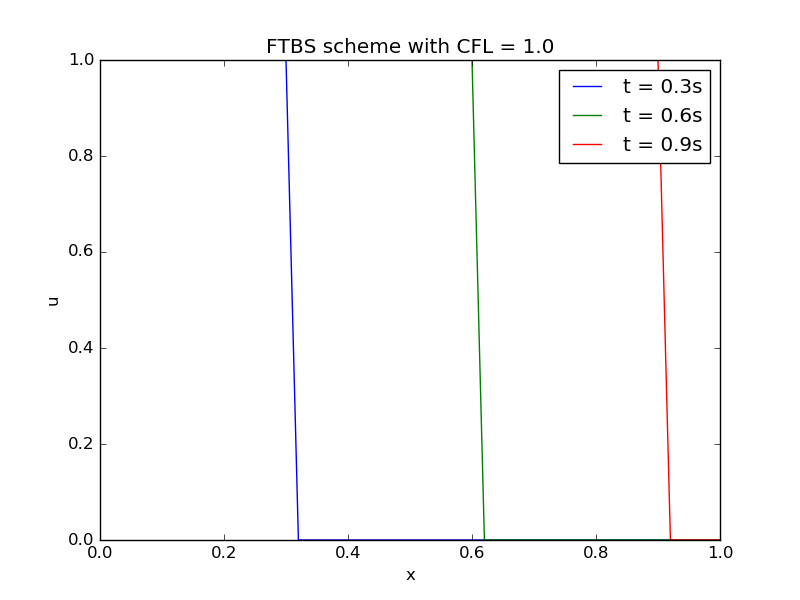
\includegraphics[width = 0.8\textwidth]{FTBS1_1_1.png}
 \caption{Plot of u v/s x for various t}
\end{figure}

We see that the function propogates without any change in its shape. Though the shape should technically be a step function
the figure shown is that of a ramp. This can be improved by decreasing the grid size.

\subsubsection{CFL = 1.2}
\begin{figure}[H]
 \centering
 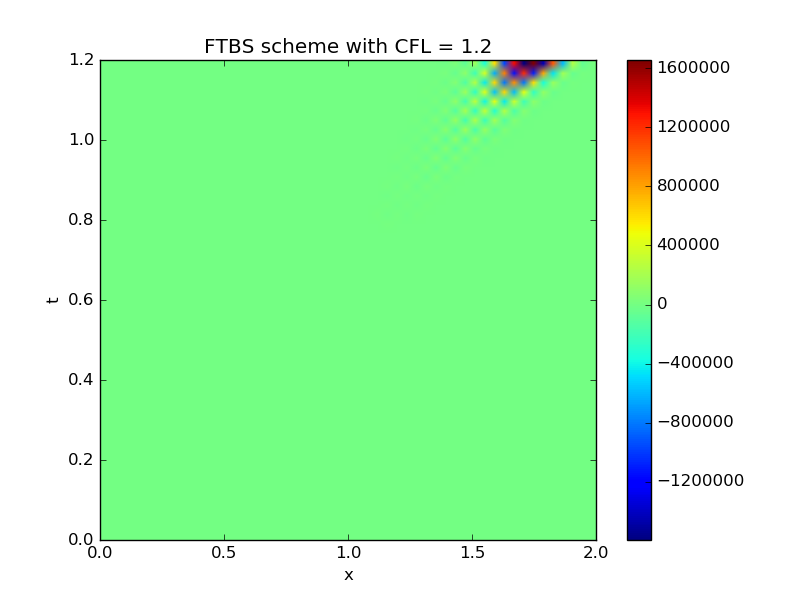
\includegraphics[width = 0.8\textwidth]{FTBS1_12.png}
 \caption{Color represents the magnitude of u at the given x and t}
\end{figure}

\begin{figure}[H]
 \centering
 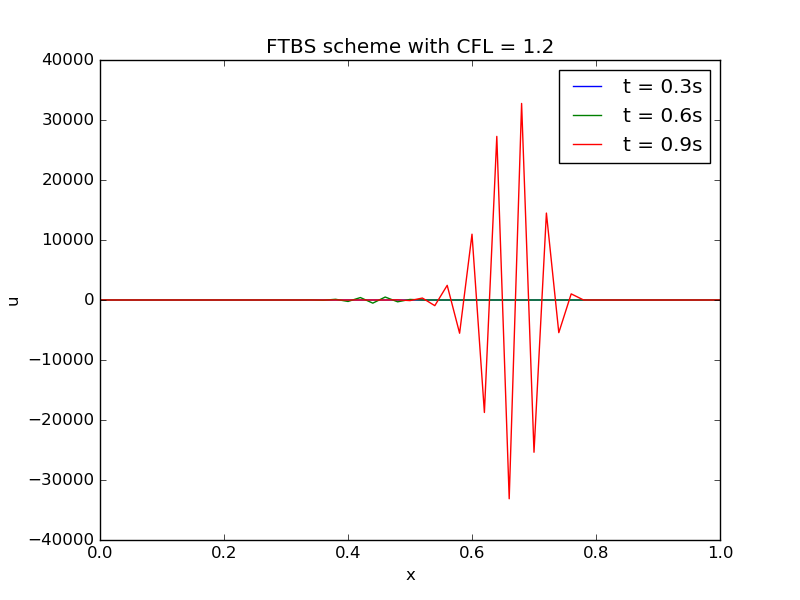
\includegraphics[width = 0.8\textwidth]{FTBS1_12_1.png}
 \caption{Plot of u v/s x for various t}
\end{figure}

\begin{figure}[H]
 \centering
 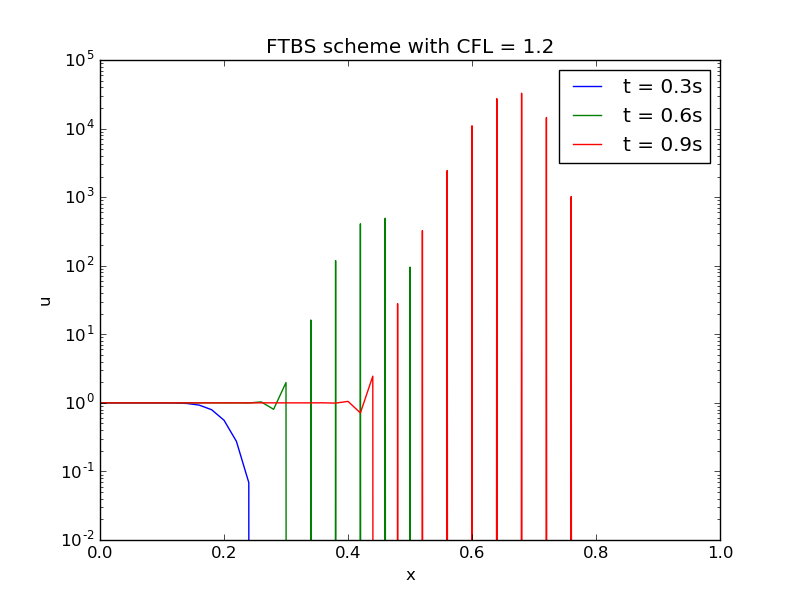
\includegraphics[width = 0.8\textwidth]{FTBS1_12_1_log.png}
 \caption{Plot of u v/s x for various t in log scale}
\end{figure}
We see that the solution diverges to very high values with time. i,e solution isn't stable

\subsection{FTFS}
\subsubsection{CFL = 0.8}
\begin{figure}[H]
 \centering
 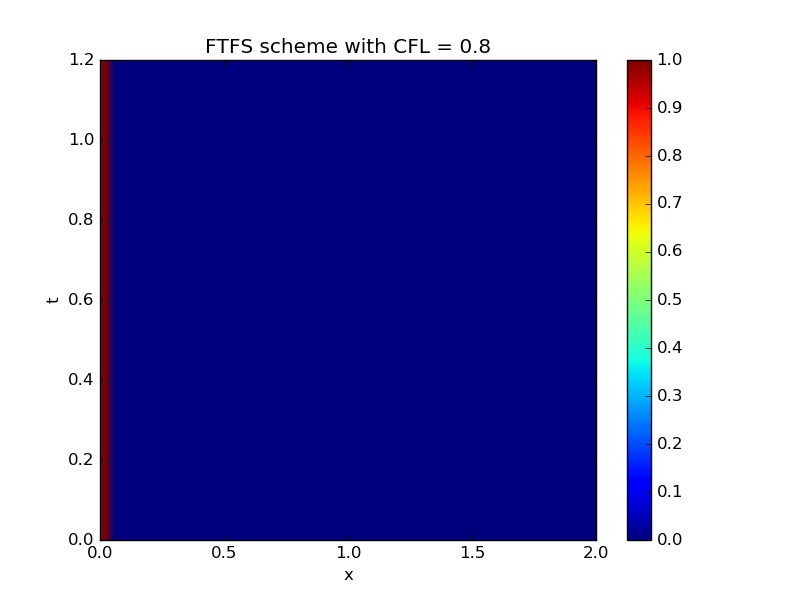
\includegraphics[width = 0.8\textwidth]{FTFS1_08.png}
 \caption{Color represents the magnitude of u at the given x and t}
\end{figure}

\begin{figure}[H]
 \centering
 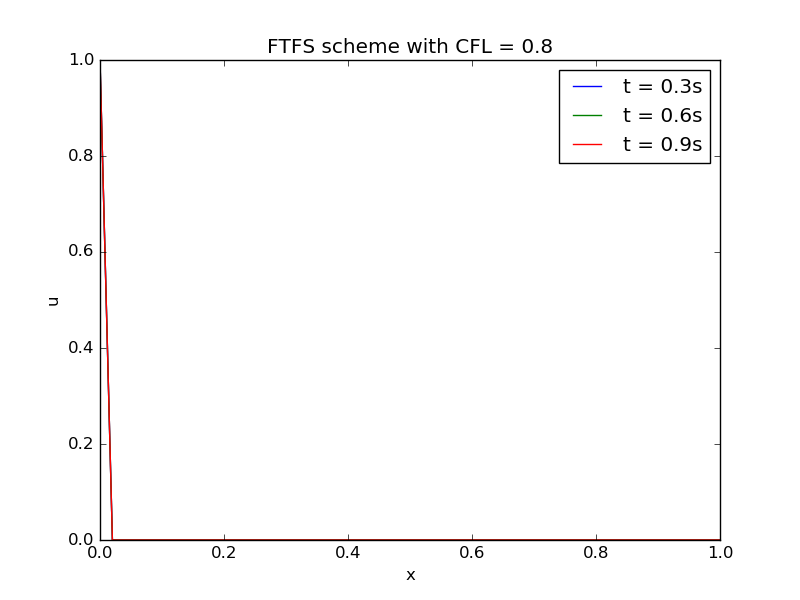
\includegraphics[width = 0.8\textwidth]{FTFS1_08_1.png}
 \caption{Plot of u v/s x for various t}
\end{figure}

\subsubsection{CFL = 1.0}
\begin{figure}[H]
 \centering
 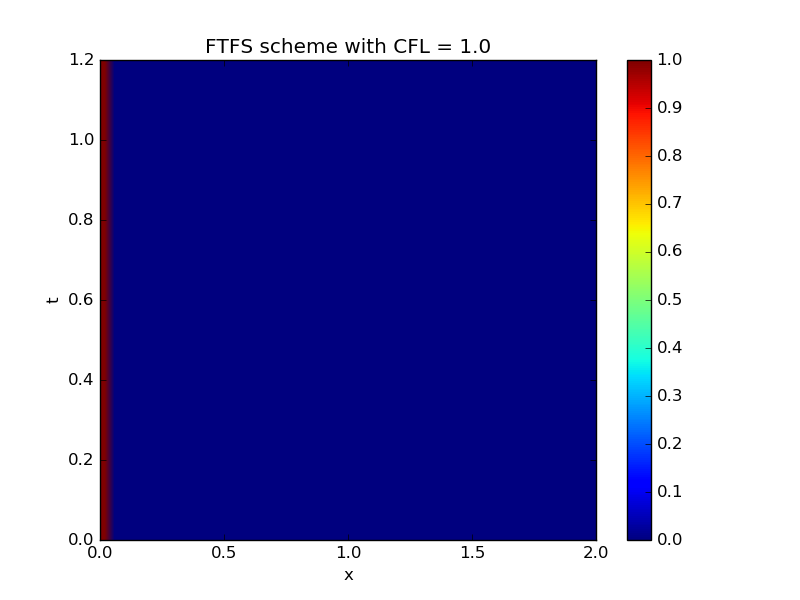
\includegraphics[width = 0.8\textwidth]{FTFS1_1.png}
 \caption{Color represents the magnitude of u at the given x and t}
\end{figure}

\begin{figure}[H]
 \centering
 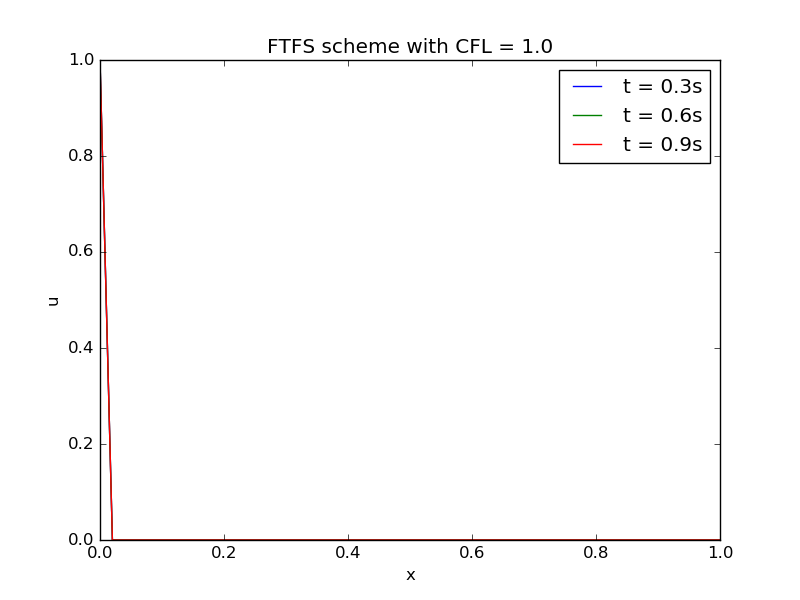
\includegraphics[width = 0.8\textwidth]{FTFS1_1_1.png}
 \caption{Plot of u v/s x for various t}
\end{figure}

\subsubsection{CFL = 1.2}
\begin{figure}[H]
 \centering
 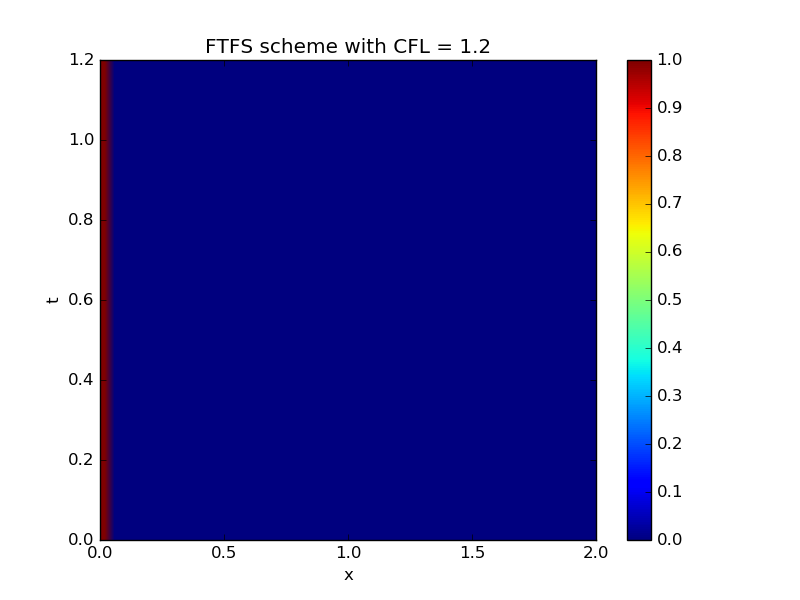
\includegraphics[width = 0.8\textwidth]{FTFS1_12.png}
 \caption{Color represents the magnitude of u at the given x and t}
\end{figure}

\begin{figure}[H]
 \centering
 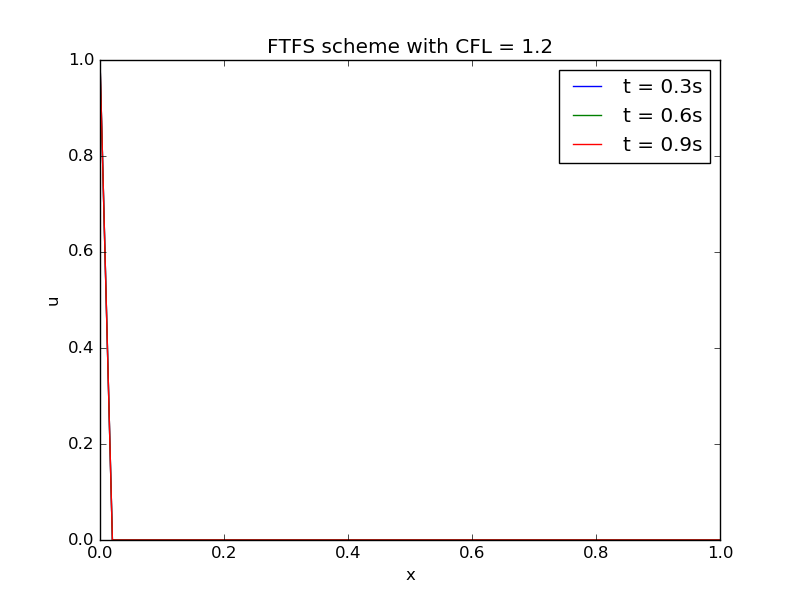
\includegraphics[width = 0.8\textwidth]{FTFS1_12_1.png}
 \caption{Plot of u v/s x for various t}
\end{figure}

We see that the solution doesn't propogate at all under FTFS. This is because the initial condition is set to xero at all points

\subsection{FTCS}
\subsubsection{CFL = 0.8}
\begin{figure}[H]
 \centering
 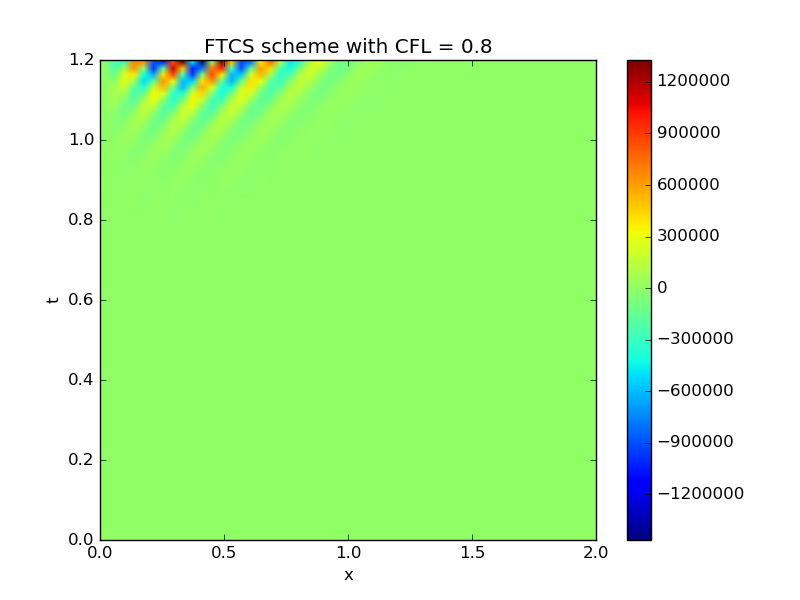
\includegraphics[width = 0.8\textwidth]{FTCS1_08.png}
 \caption{Color represents the magnitude of u at the given x and t}
\end{figure}

\begin{figure}[H]
 \centering
 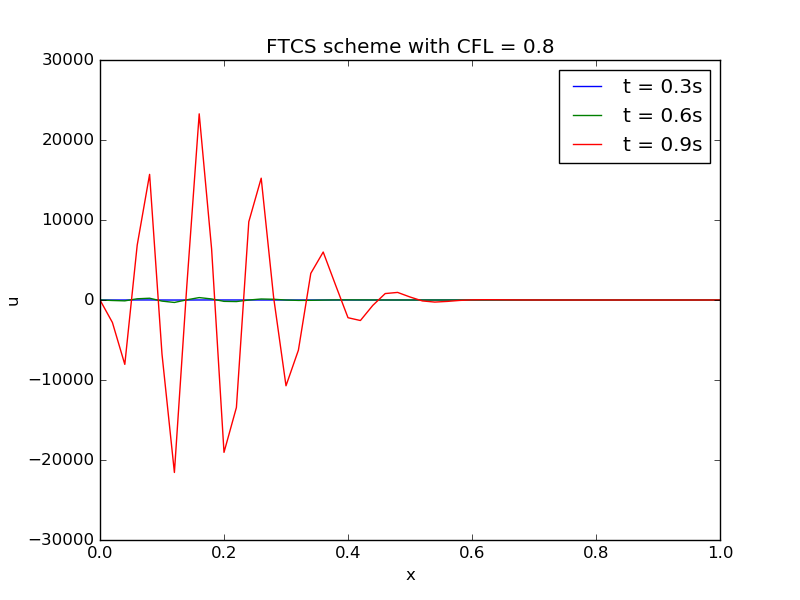
\includegraphics[width = 0.8\textwidth]{FTCS1_08_1.png}
 \caption{Plot of u v/s x for various t}
\end{figure}

\begin{figure}[H]
 \centering
 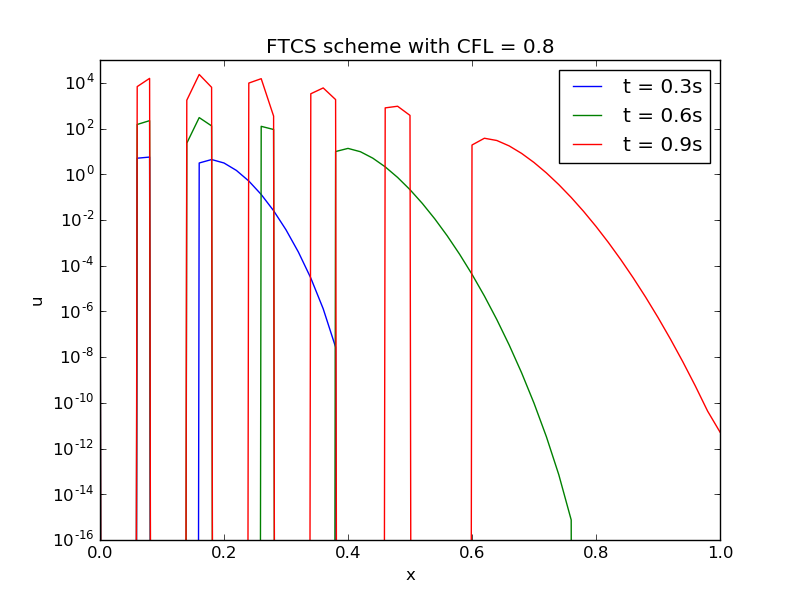
\includegraphics[width = 0.8\textwidth]{FTCS1_08_1_log.png}
 \caption{Plot of u v/s x for various t in log scale}
\end{figure}

\subsubsection{CFL = 1.0}
\begin{figure}[H]
 \centering
 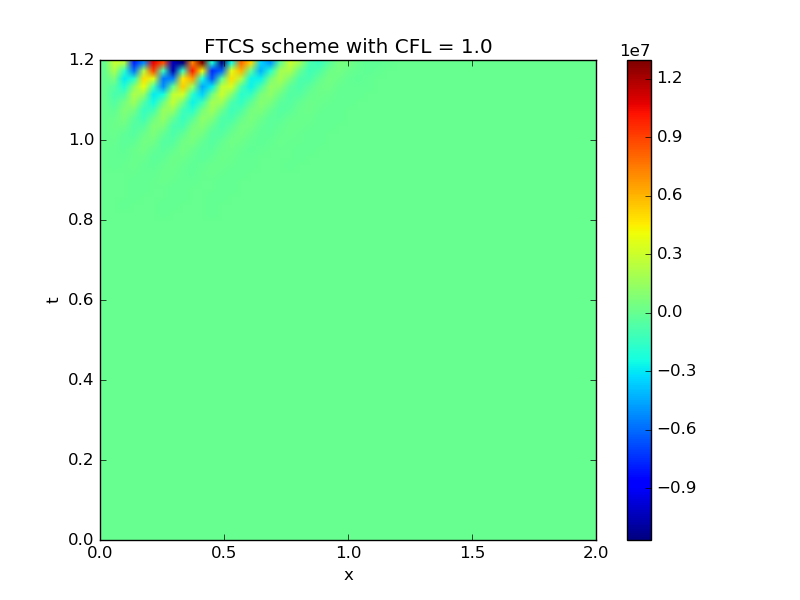
\includegraphics[width = 0.8\textwidth]{FTCS1_1.png}
 \caption{Color represents the magnitude of u at the given x and t}
\end{figure}

\begin{figure}[H]
 \centering
 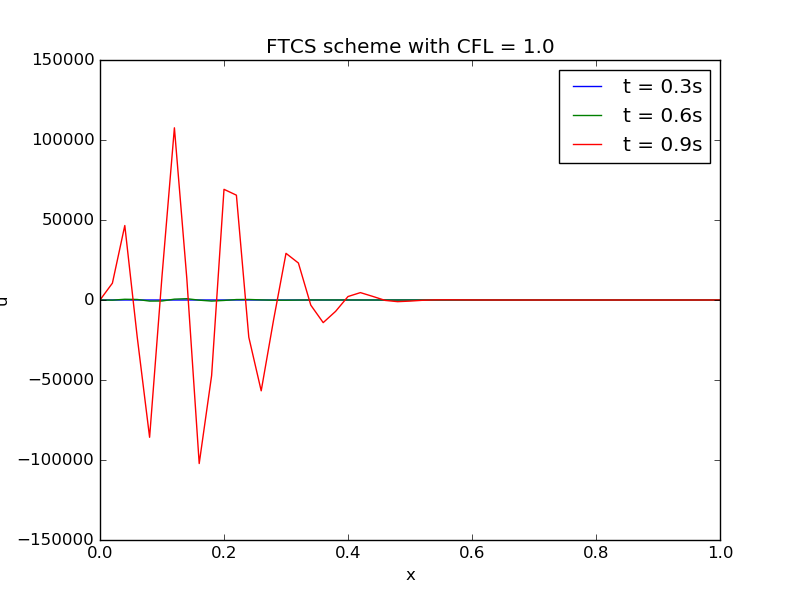
\includegraphics[width = 0.8\textwidth]{FTCS1_1_1.png}
 \caption{Plot of u v/s x for various t}
\end{figure}

\begin{figure}[H]
 \centering
 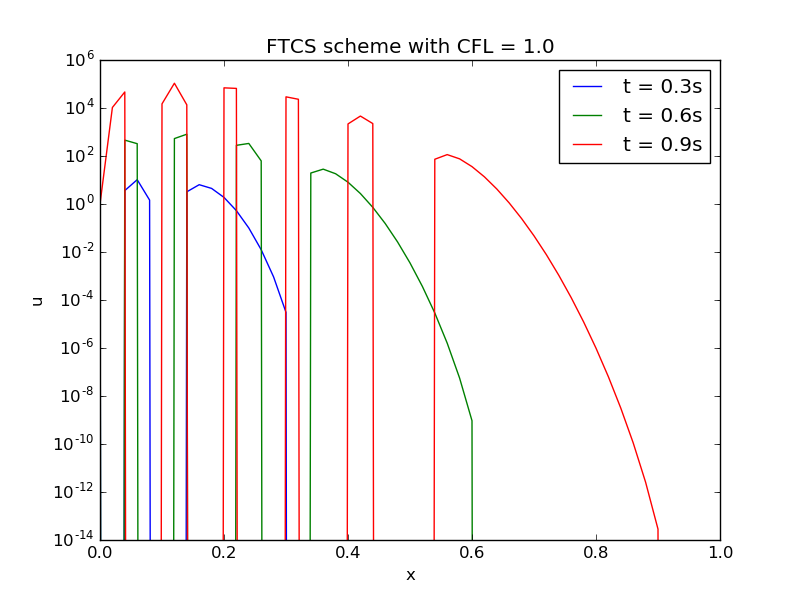
\includegraphics[width = 0.8\textwidth]{FTCS1_1_1_log.png}
 \caption{Plot of u v/s x for various t in log scale}
\end{figure}

\subsubsection{CFL = 1.2}
\begin{figure}[H]
 \centering
 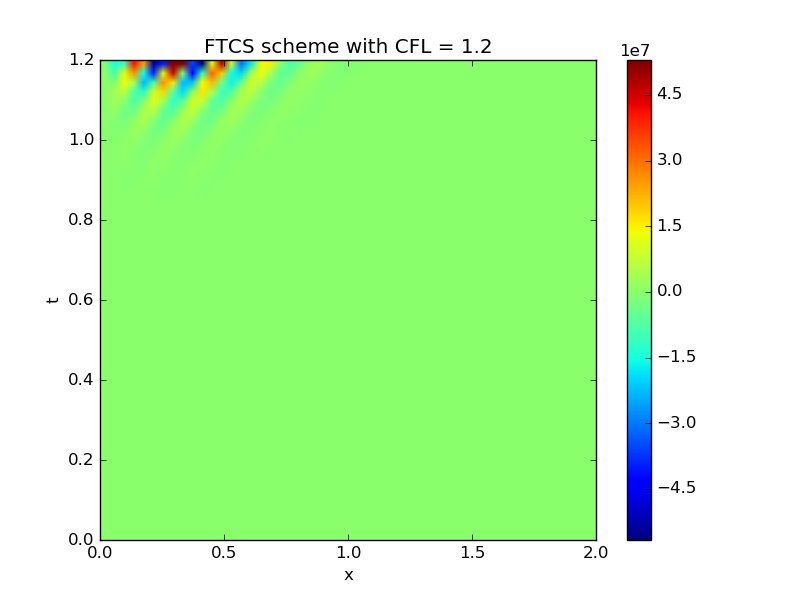
\includegraphics[width = 0.8\textwidth]{FTCS1_12.png}
 \caption{Color represents the magnitude of u at the given x and t}
\end{figure}

\begin{figure}[H]
 \centering
 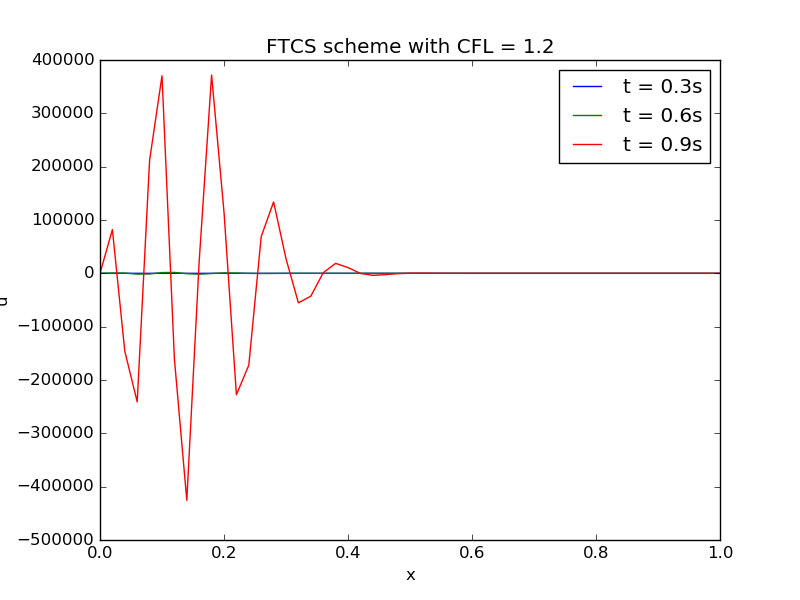
\includegraphics[width = 0.8\textwidth]{FTCS1_12_1.png}
 \caption{Plot of u v/s x for various t}
\end{figure}

\begin{figure}[H]
 \centering
 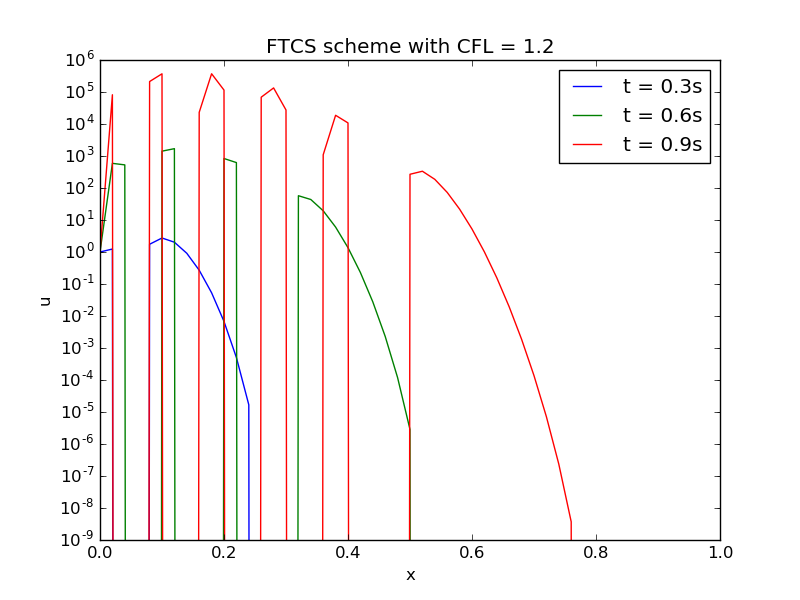
\includegraphics[width = 0.8\textwidth]{FTCS1_12_1_log.png}
 \caption{Plot of u v/s x for various t in log scale}
\end{figure}

We see that the solution diverges for all CFL values.

\section{Question 2:}
In this question we solve the linear wave equation when the initial condition is a sine wave and/or a combination of sine waves

\subsection{Single frequency}
\subsubsection{FTBS}
\subsubsubsection{CFL = 0.8}
\begin{figure}[H]
 \centering
 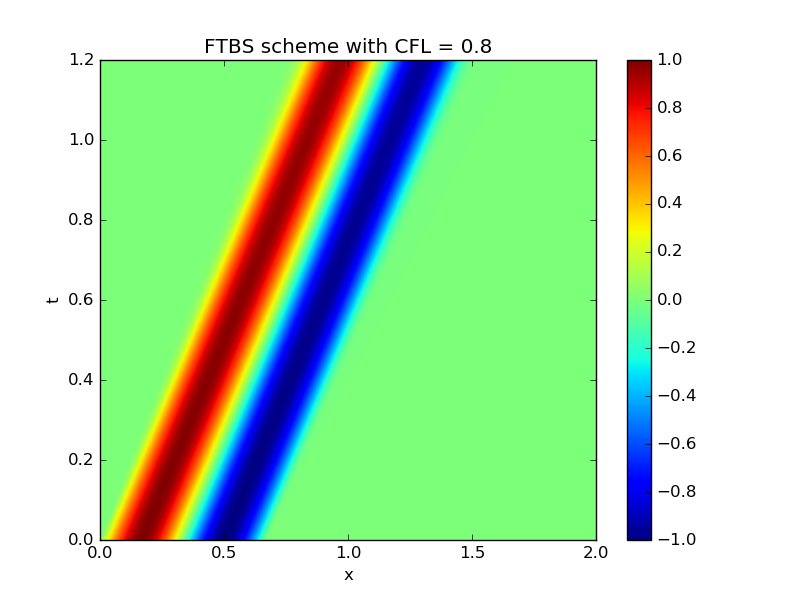
\includegraphics[width = 0.8\textwidth]{FTBS2_08.png}
 \caption{Color represents the magnitude of u at the given x and t}
\end{figure}

\begin{figure}[H]
 \centering
 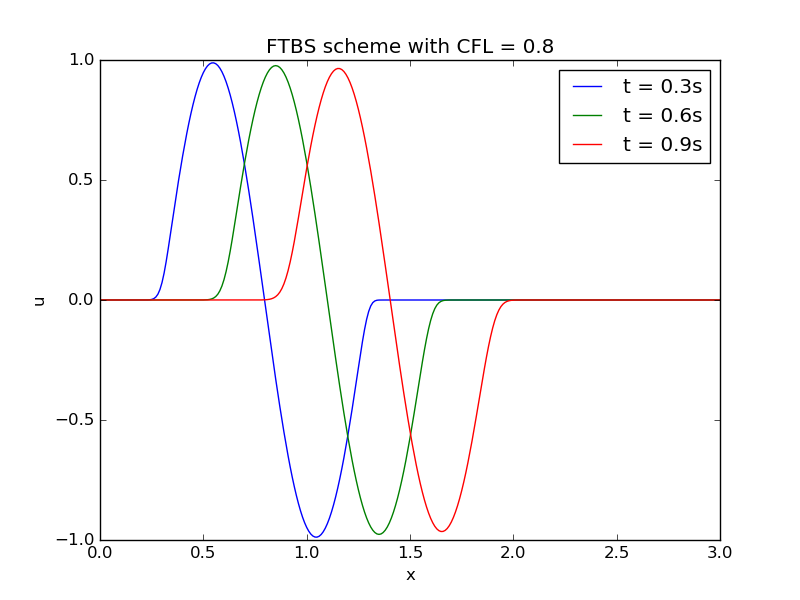
\includegraphics[width = 0.8\textwidth]{FTBS2_08_1.png}
 \caption{Plot of u v/s x for various t}
\end{figure}

We see that that the function starts smoothening and also dampens with time.

\subsubsection{CFL = 1.0}
\begin{figure}[H]
 \centering
 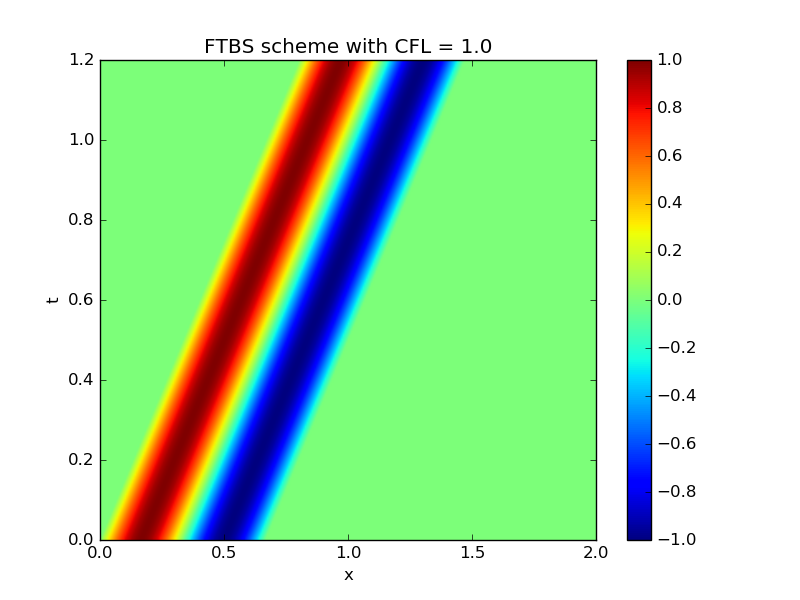
\includegraphics[width = 0.8\textwidth]{FTBS2_1.png}
 \caption{Color represents the magnitude of u at the given x and t}
\end{figure}

\begin{figure}[H]
 \centering
 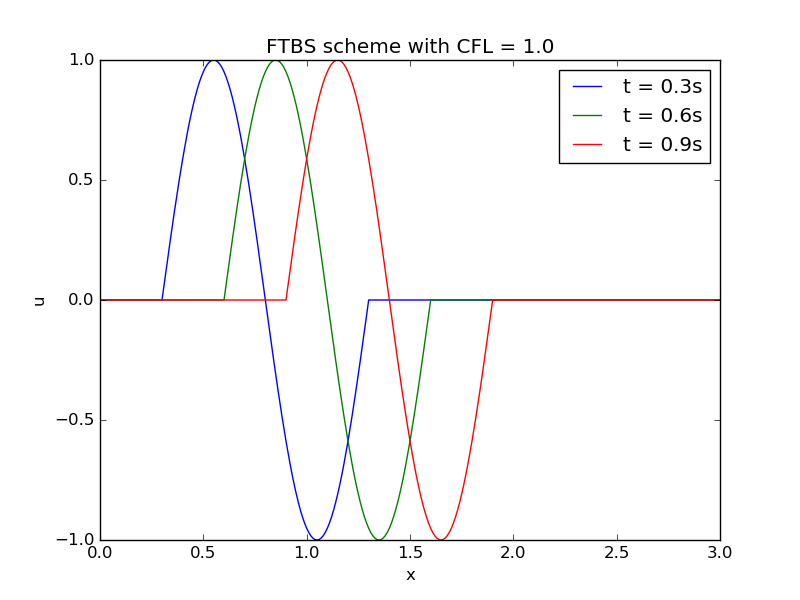
\includegraphics[width = 0.8\textwidth]{FTBS2_1_1.png}
 \caption{Plot of u v/s x for various t}
\end{figure}

The sine wave propogates without any damping.


\subsubsection{CFL = 1.2}
\begin{figure}[H]
 \centering
 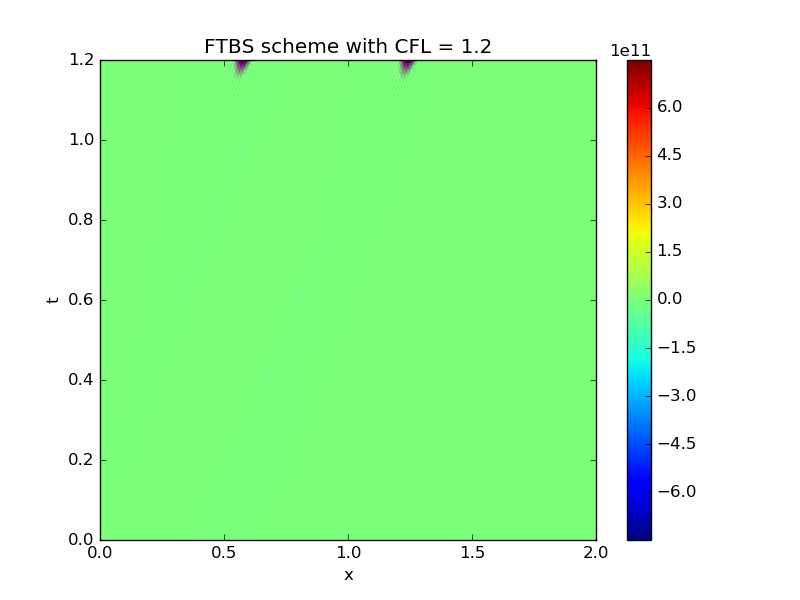
\includegraphics[width = 0.8\textwidth]{FTBS2_12.png}
 \caption{Color represents the magnitude of u at the given x and t}
\end{figure}

\begin{figure}[H]
 \centering
 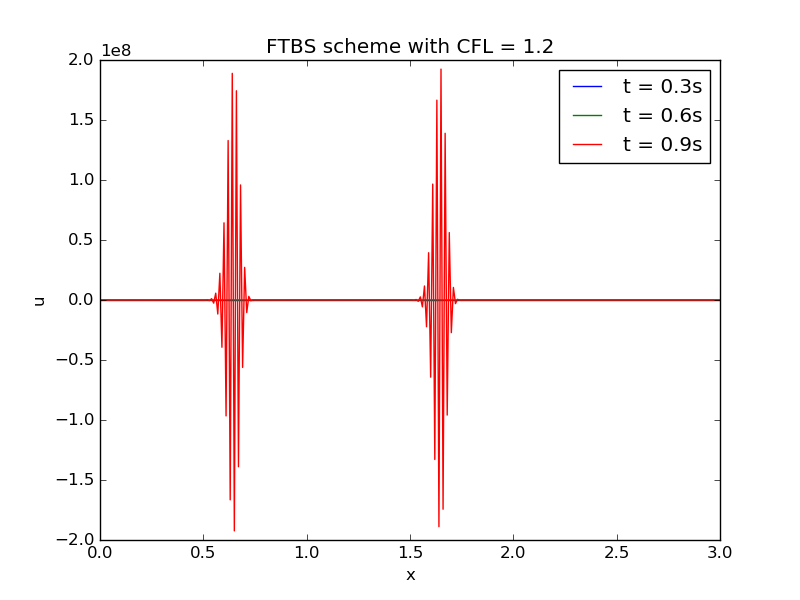
\includegraphics[width = 0.8\textwidth]{FTBS2_12_1.png}
 \caption{Plot of u v/s x for various t}
\end{figure}

\begin{figure}[H]
 \centering
 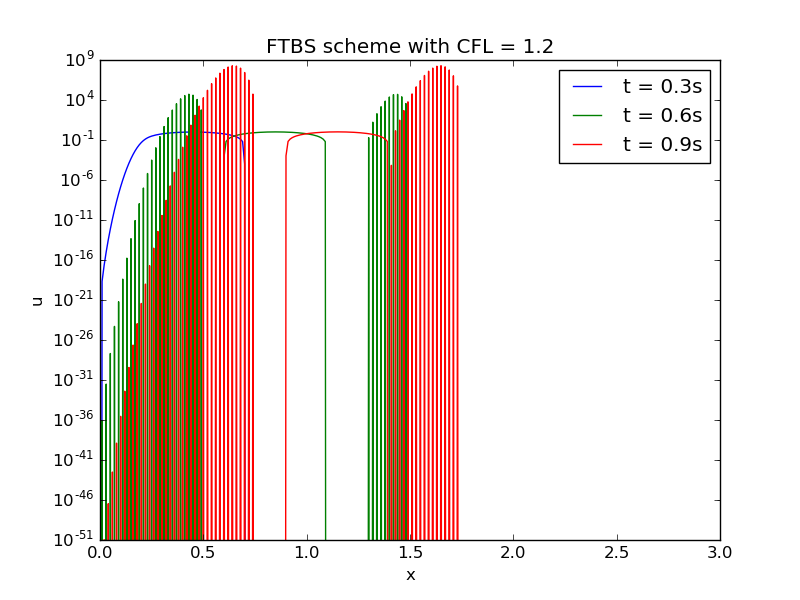
\includegraphics[width = 0.8\textwidth]{FTBS2_12_1_log.png}
 \caption{Plot of u v/s x for various t in log scale}
\end{figure}
We see that the solution diverges to very high values with time. i,e solution isn't stable

\subsection{FTFS}
\subsubsection{CFL = 0.8}
\begin{figure}[H]
 \centering
 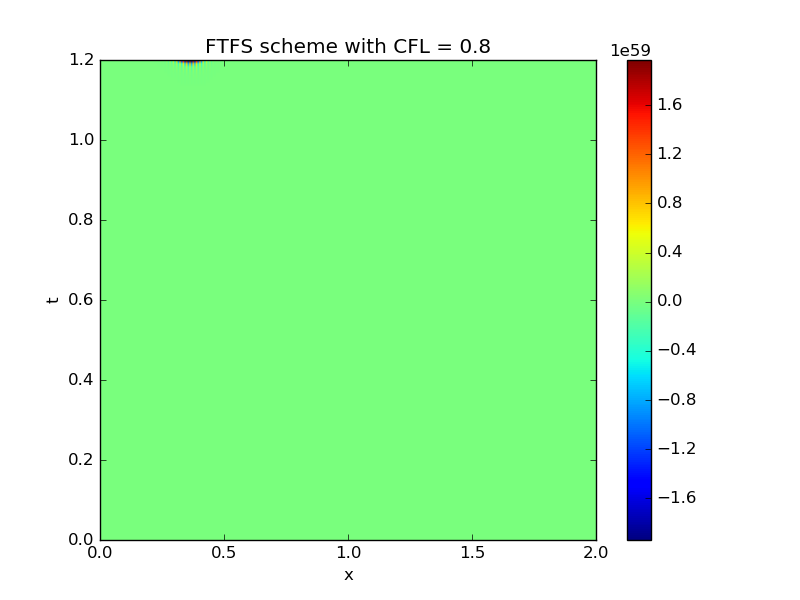
\includegraphics[width = 0.8\textwidth]{FTFS2_08.png}
 \caption{Color represents the magnitude of u at the given x and t}
\end{figure}

\begin{figure}[H]
 \centering
 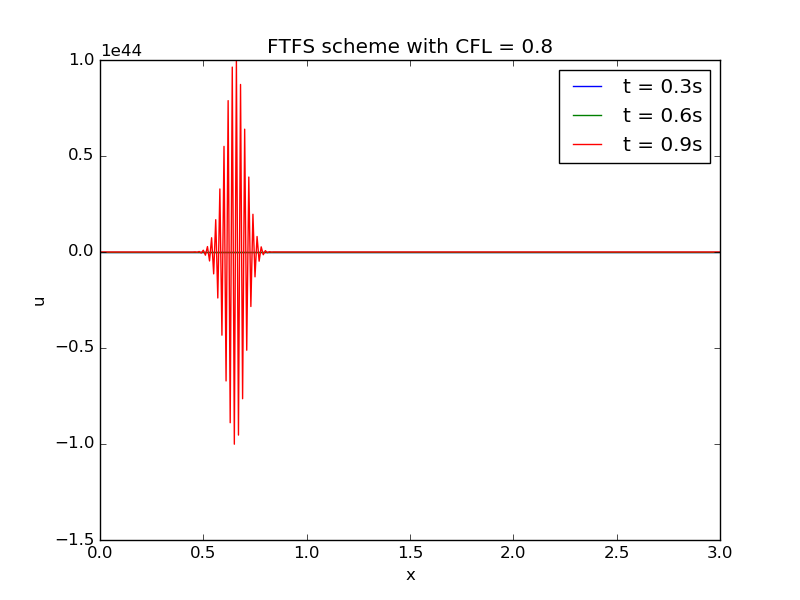
\includegraphics[width = 0.8\textwidth]{FTFS2_08_1.png}
 \caption{Plot of u v/s x for various t}
\end{figure}

\subsubsection{CFL = 1.0}
\begin{figure}[H]
 \centering
 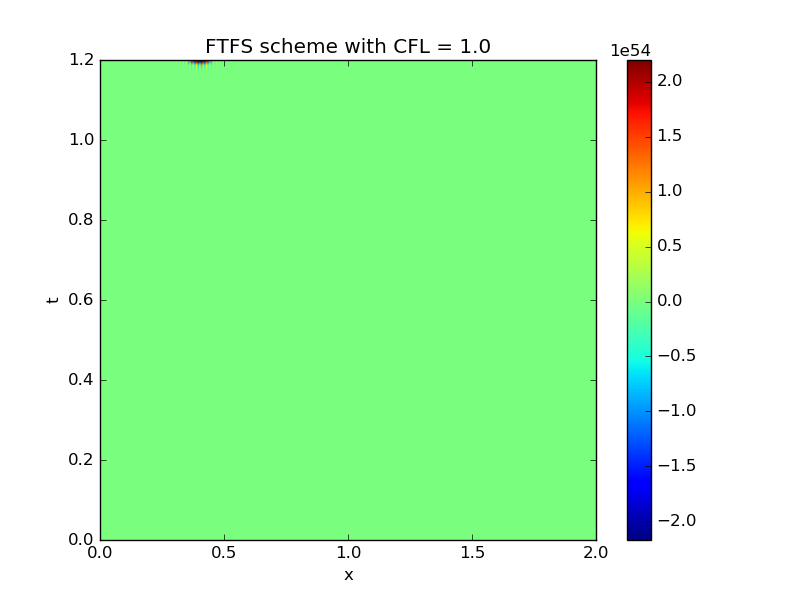
\includegraphics[width = 0.8\textwidth]{FTFS2_1.png}
 \caption{Color represents the magnitude of u at the given x and t}
\end{figure}

\begin{figure}[H]
 \centering
 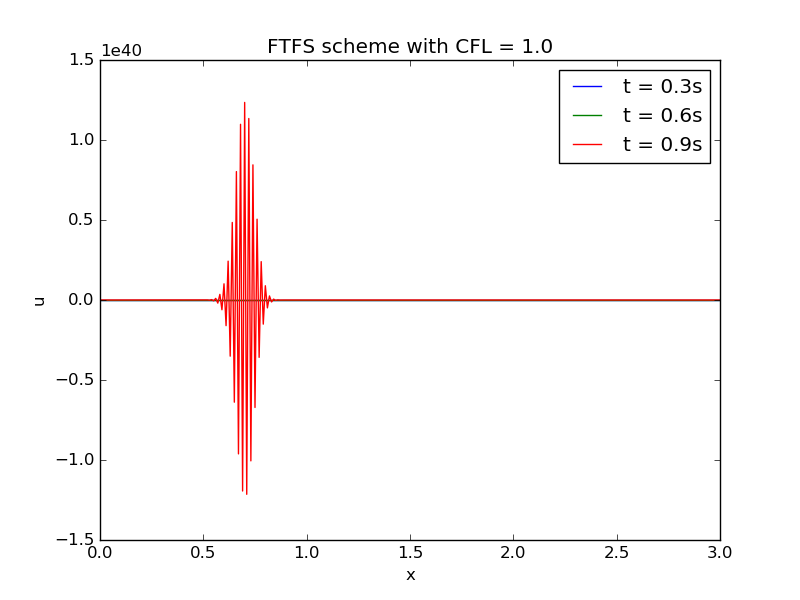
\includegraphics[width = 0.8\textwidth]{FTFS2_1_1.png}
 \caption{Plot of u v/s x for various t}
\end{figure}

\subsubsection{CFL = 1.2}
\begin{figure}[H]
 \centering
 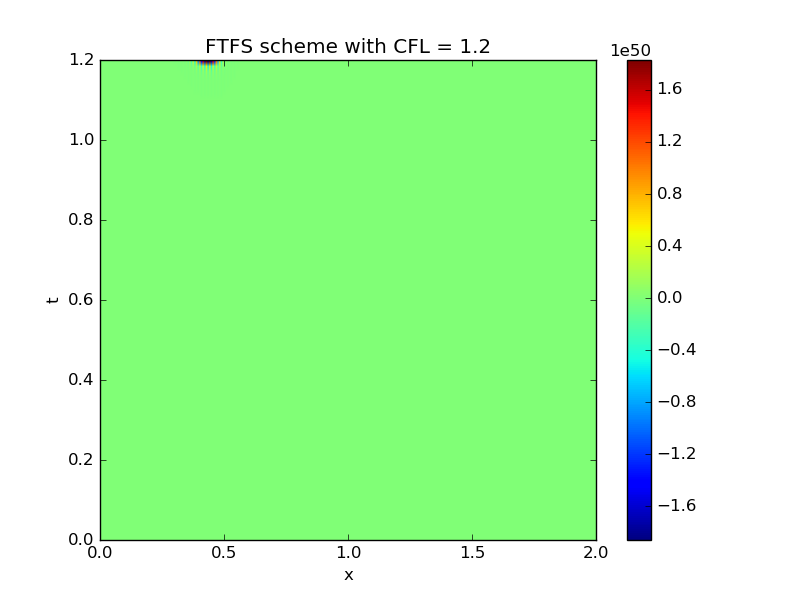
\includegraphics[width = 0.8\textwidth]{FTFS2_12.png}
 \caption{Color represents the magnitude of u at the given x and t}
\end{figure}

\begin{figure}[H]
 \centering
 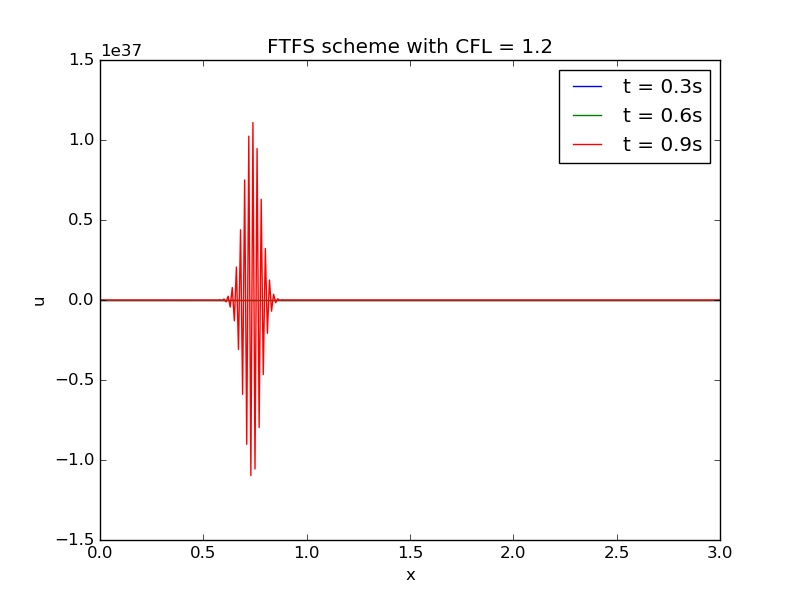
\includegraphics[width = 0.8\textwidth]{FTFS2_12_1.png}
 \caption{Plot of u v/s x for various t}
\end{figure}

We see that the solution diverges i.e the scheme is unstable

\subsection{FTCS}
\subsubsection{CFL = 0.8}
\begin{figure}[H]
 \centering
 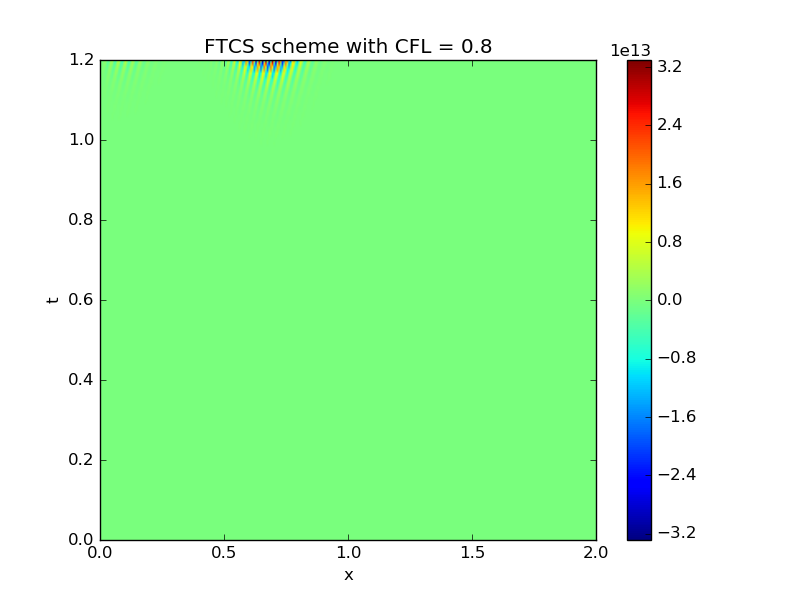
\includegraphics[width = 0.8\textwidth]{FTCS2_08.png}
 \caption{Color represents the magnitude of u at the given x and t}
\end{figure}

\begin{figure}[H]
 \centering
 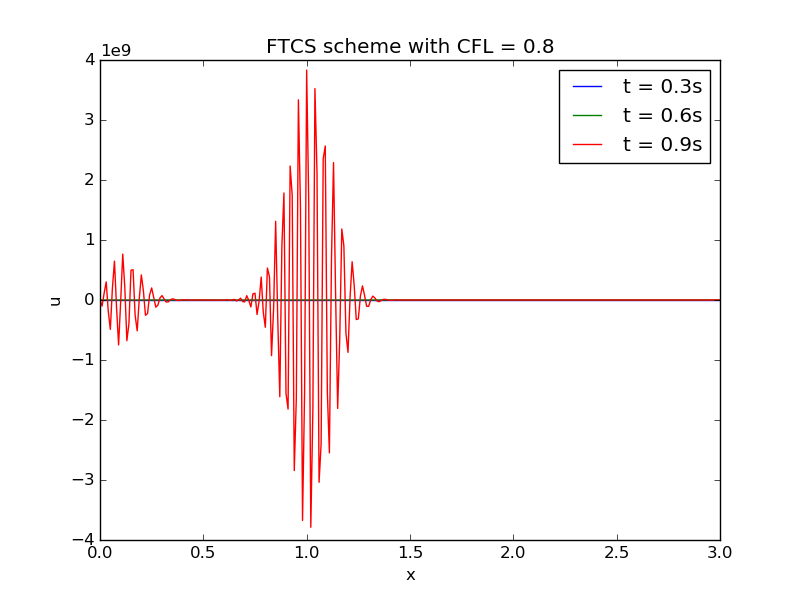
\includegraphics[width = 0.8\textwidth]{FTCS2_08_1.png}
 \caption{Plot of u v/s x for various t}
\end{figure}

\begin{figure}[H]
 \centering
 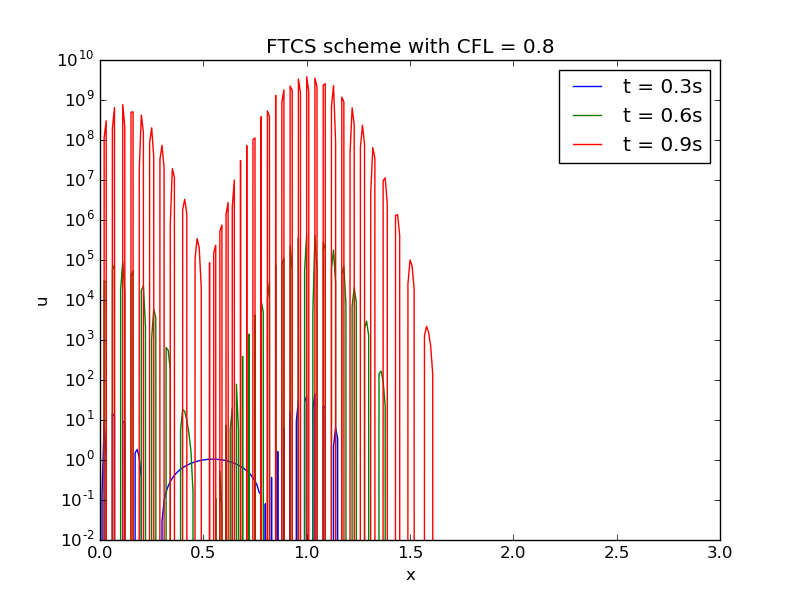
\includegraphics[width = 0.8\textwidth]{FTCS2_08_1_log.png}
 \caption{Plot of u v/s x for various t in log scale}
\end{figure}

\subsubsection{CFL = 1.0}
\begin{figure}[H]
 \centering
 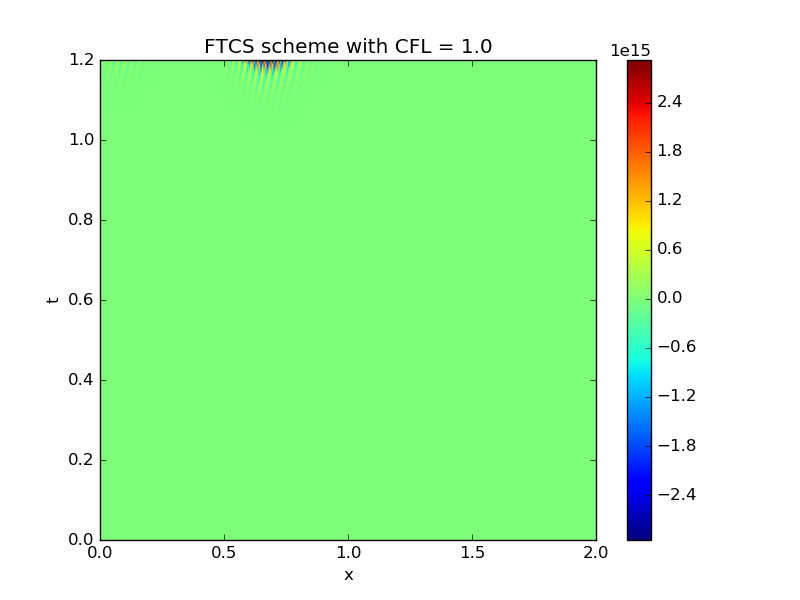
\includegraphics[width = 0.8\textwidth]{FTCS2_1.png}
 \caption{Color represents the magnitude of u at the given x and t}
\end{figure}

\begin{figure}[H]
 \centering
 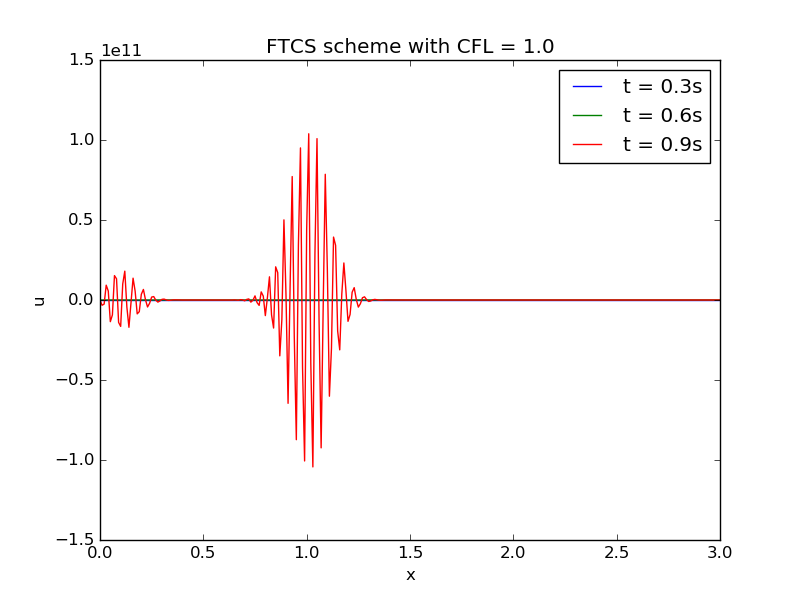
\includegraphics[width = 0.8\textwidth]{FTCS2_1_1.png}
 \caption{Plot of u v/s x for various t}
\end{figure}

\begin{figure}[H]
 \centering
 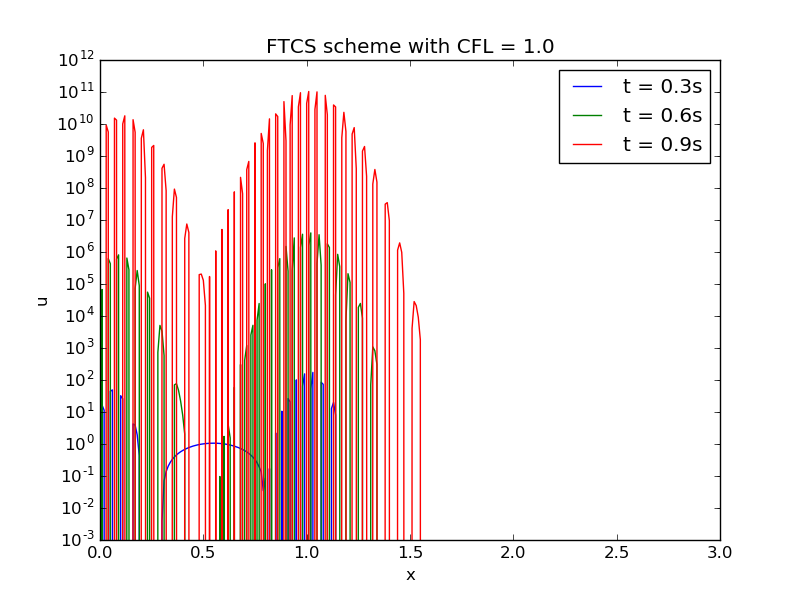
\includegraphics[width = 0.8\textwidth]{FTCS2_1_1_log.png}
 \caption{Plot of u v/s x for various t in log scale}
\end{figure}

\subsubsection{CFL = 1.2}
\begin{figure}[H]
 \centering
 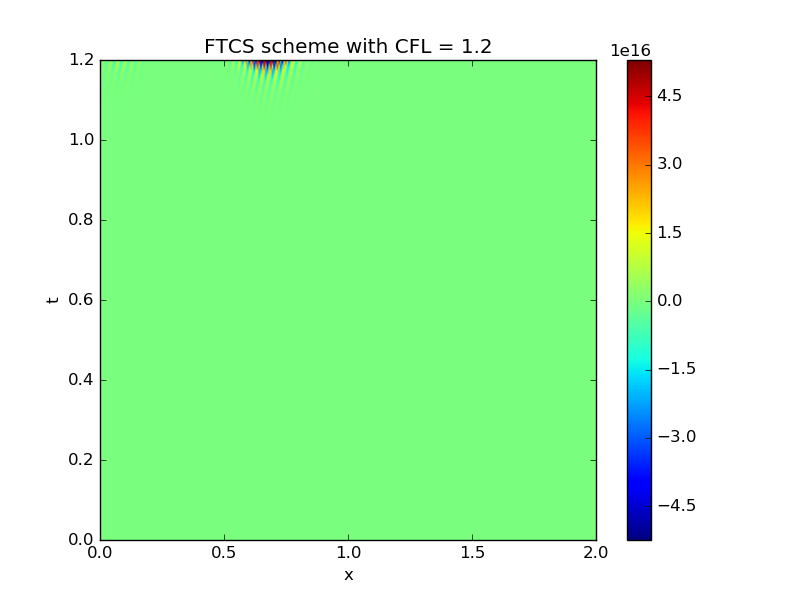
\includegraphics[width = 0.8\textwidth]{FTCS2_12.png}
 \caption{Color represents the magnitude of u at the given x and t}
\end{figure}

\begin{figure}[H]
 \centering
 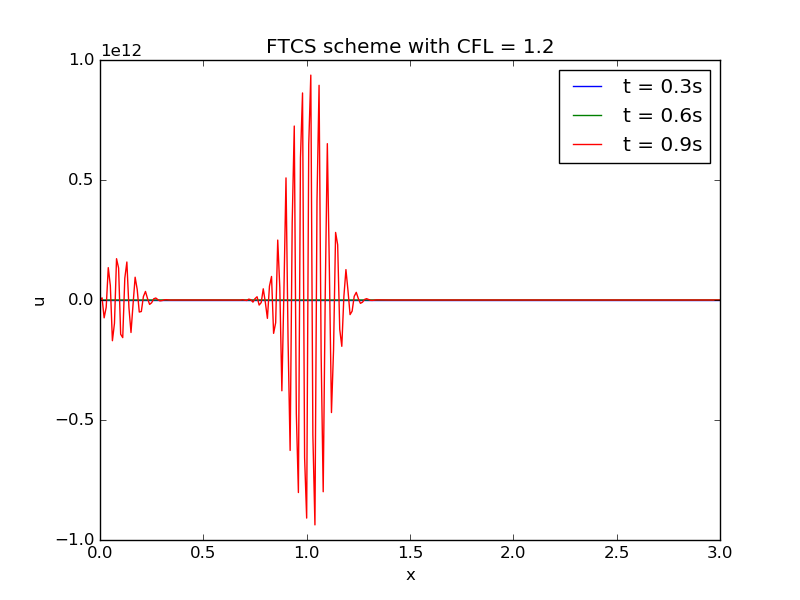
\includegraphics[width = 0.8\textwidth]{FTCS2_12_1.png}
 \caption{Plot of u v/s x for various t}
\end{figure}

\begin{figure}[H]
 \centering
 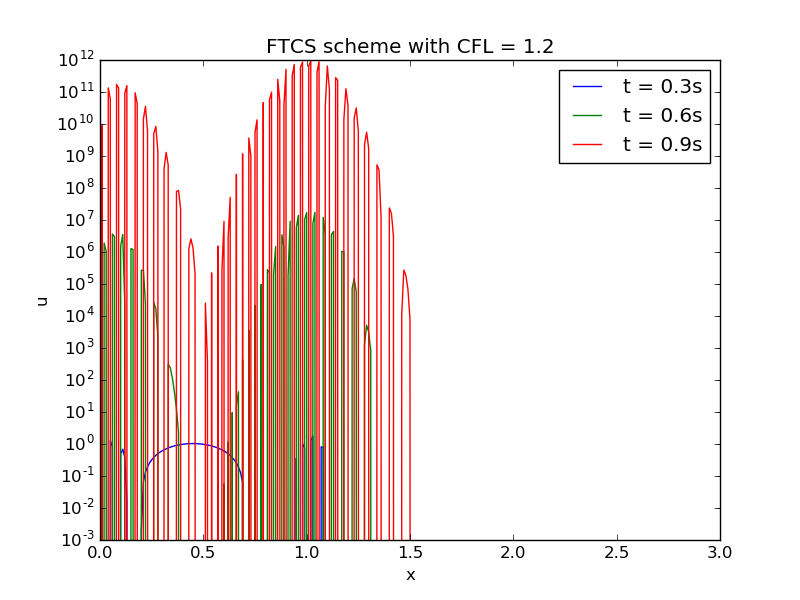
\includegraphics[width = 0.8\textwidth]{FTCS2_12_1_log.png}
 \caption{Plot of u v/s x for various t in log scale}
\end{figure}

We see that the solution doesn't converge.
\subsection{Multiple frequencies}
\subsubsection{FTBS}
\subsubsubsection{CFL = 0.8}
\begin{figure}[H]
 \centering
 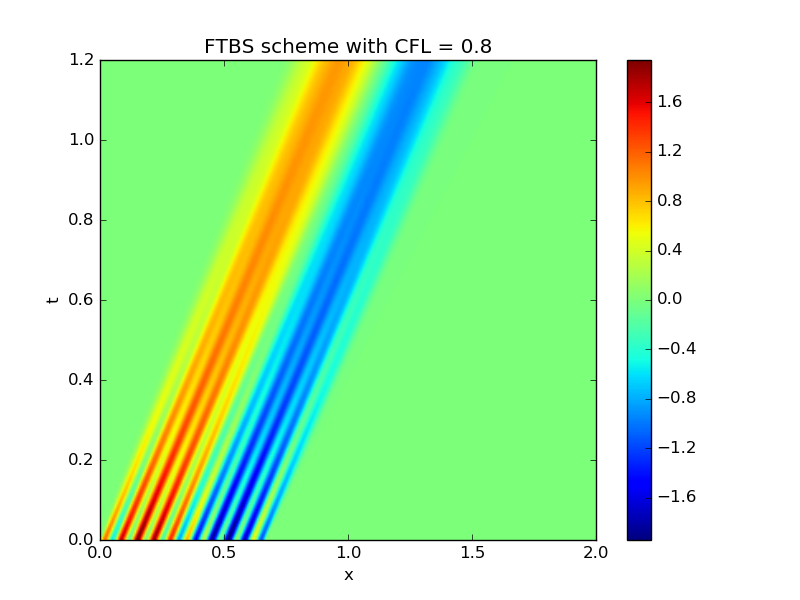
\includegraphics[width = 0.8\textwidth]{FTBS3_08.png}
 \caption{Color represents the magnitude of u at the given x and t}
\end{figure}

\begin{figure}[H]
 \centering
 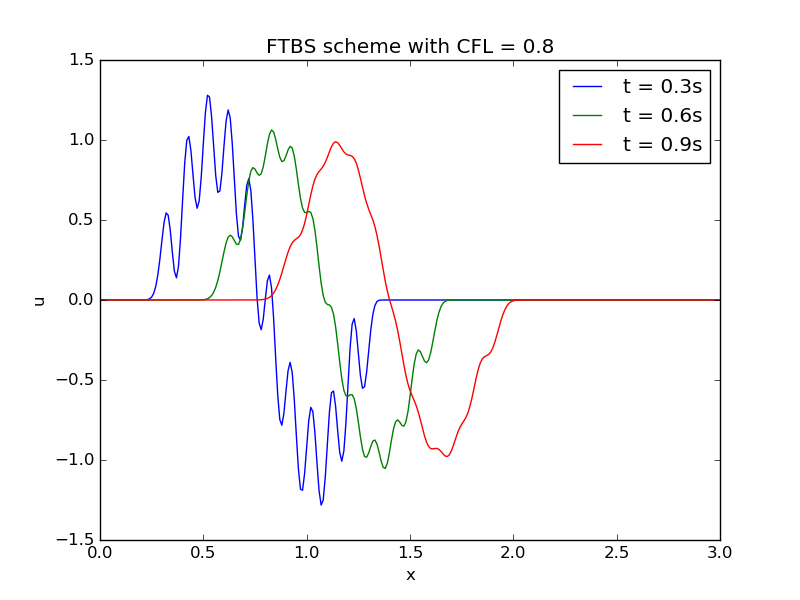
\includegraphics[width = 0.8\textwidth]{FTBS3_08_1.png}
 \caption{Plot of u v/s x for various t}
\end{figure}

We see that that the function starts smoothening and also dampens with time. It can also be noted that the high frequency
components dampen faster

\subsubsection{CFL = 1.0}
\begin{figure}[H]
 \centering
 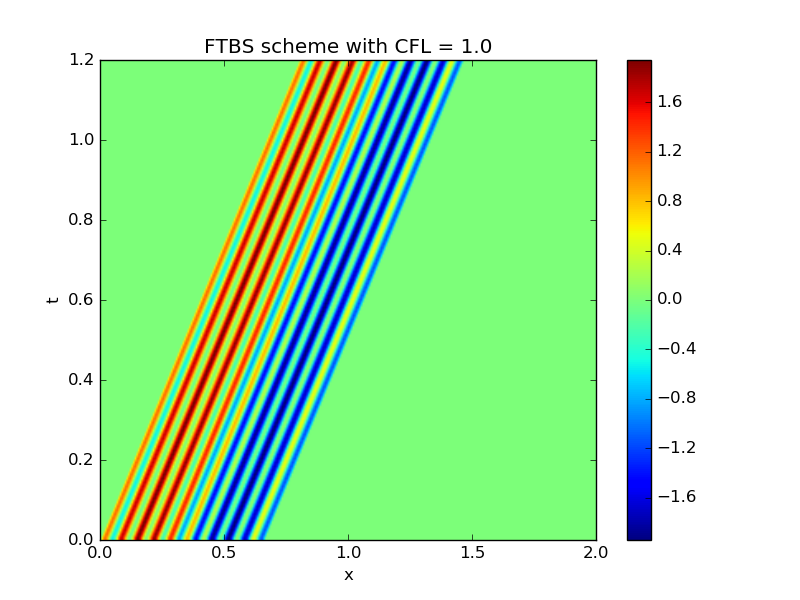
\includegraphics[width = 0.8\textwidth]{FTBS3_1.png}
 \caption{Color represents the magnitude of u at the given x and t}
\end{figure}

\begin{figure}[H]
 \centering
 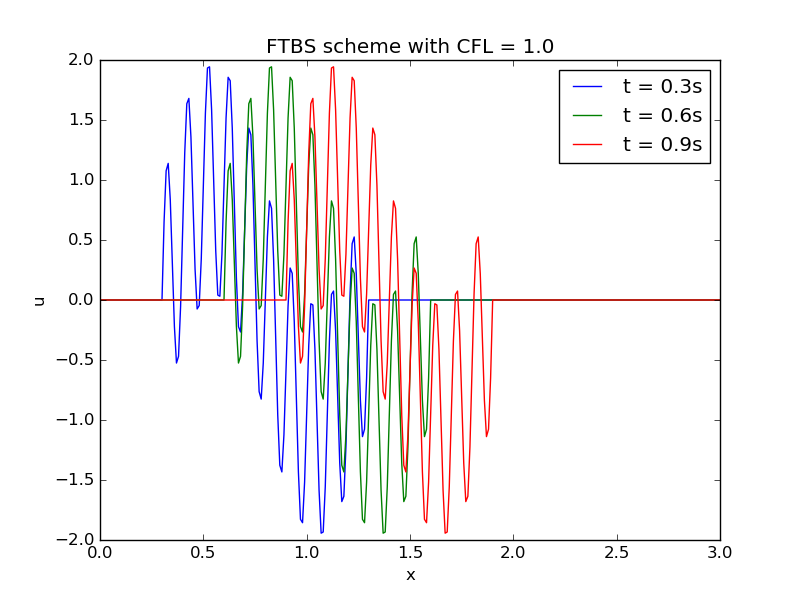
\includegraphics[width = 0.8\textwidth]{FTBS3_1_1.png}
 \caption{Plot of u v/s x for various t}
\end{figure}

The sine wave propogates without any damping.


\subsubsection{CFL = 1.2}
\begin{figure}[H]
 \centering
 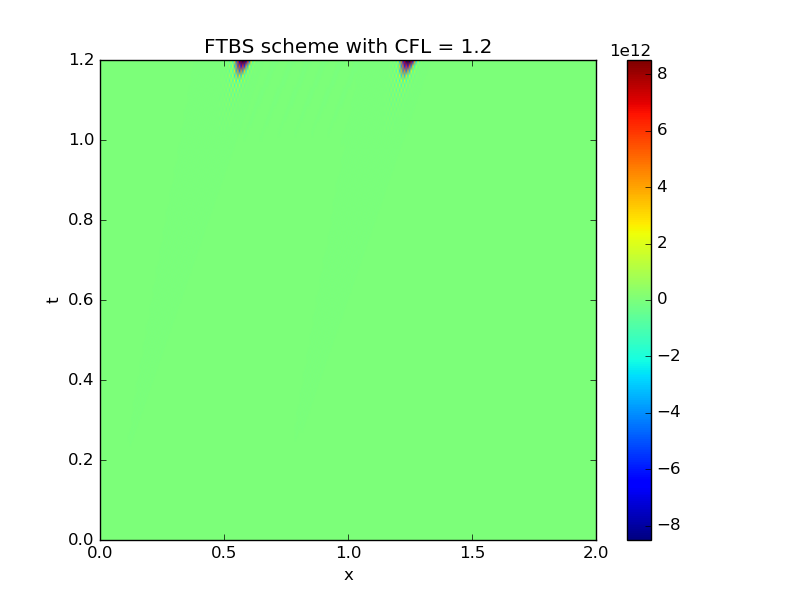
\includegraphics[width = 0.8\textwidth]{FTBS3_12.png}
 \caption{Color represents the magnitude of u at the given x and t}
\end{figure}

\begin{figure}[H]
 \centering
 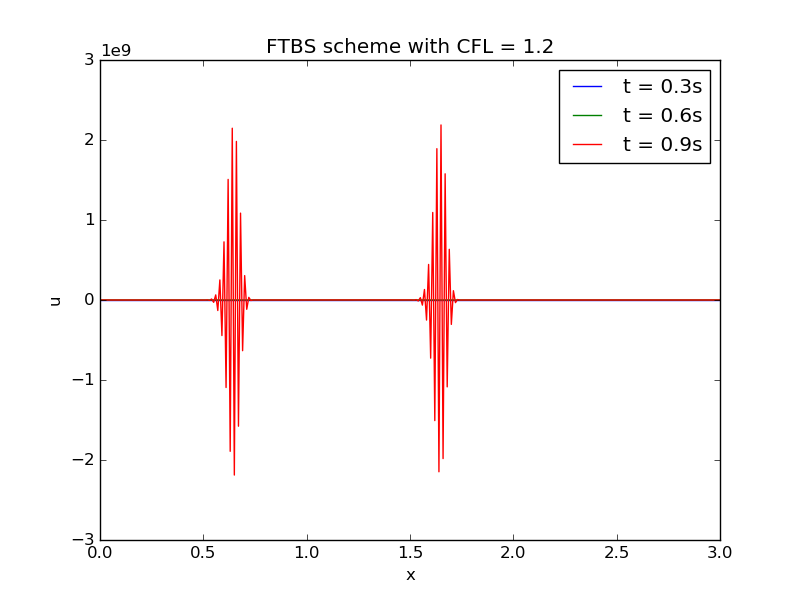
\includegraphics[width = 0.8\textwidth]{FTBS3_12_1.png}
 \caption{Plot of u v/s x for various t}
\end{figure}

\begin{figure}[H]
 \centering
 \includegraphics[width = 0.8\textwidth]{FTBS3_12_1_log.png}
 \caption{Plot of u v/s x for various t in log scale}
\end{figure}
We see that the solution diverges to very high values with time. i,e solution isn't stable

\subsection{FTFS}
\subsubsection{CFL = 0.8}
\begin{figure}[H]
 \centering
 \includegraphics[width = 0.8\textwidth]{FTFS3_08.png}
 \caption{Color represents the magnitude of u at the given x and t}
\end{figure}

\begin{figure}[H]
 \centering
 \includegraphics[width = 0.8\textwidth]{FTFS3_08_1.png}
 \caption{Plot of u v/s x for various t}
\end{figure}

\subsubsection{CFL = 1.0}
\begin{figure}[H]
 \centering
 \includegraphics[width = 0.8\textwidth]{FTFS3_1.png}
 \caption{Color represents the magnitude of u at the given x and t}
\end{figure}

\begin{figure}[H]
 \centering
 \includegraphics[width = 0.8\textwidth]{FTFS3_1_1.png}
 \caption{Plot of u v/s x for various t}
\end{figure}

\subsubsection{CFL = 1.2}
\begin{figure}[H]
 \centering
 \includegraphics[width = 0.8\textwidth]{FTFS3_12.png}
 \caption{Color represents the magnitude of u at the given x and t}
\end{figure}

\begin{figure}[H]
 \centering
 \includegraphics[width = 0.8\textwidth]{FTFS3_12_1.png}
 \caption{Plot of u v/s x for various t}
\end{figure}

We see that the solution diverges i.e the scheme is unstable

\subsection{FTCS}
\subsubsection{CFL = 0.8}
\begin{figure}[H]
 \centering
 \includegraphics[width = 0.8\textwidth]{FTCS3_08.png}
 \caption{Color represents the magnitude of u at the given x and t}
\end{figure}

\begin{figure}[H]
 \centering
 \includegraphics[width = 0.8\textwidth]{FTCS3_08_1.png}
 \caption{Plot of u v/s x for various t}
\end{figure}

\begin{figure}[H]
 \centering
 \includegraphics[width = 0.8\textwidth]{FTCS3_08_1_log.png}
 \caption{Plot of u v/s x for various t in log scale}
\end{figure}

\subsubsection{CFL = 1.0}
\begin{figure}[H]
 \centering
 \includegraphics[width = 0.8\textwidth]{FTCS3_1.png}
 \caption{Color represents the magnitude of u at the given x and t}
\end{figure}

\begin{figure}[H]
 \centering
 \includegraphics[width = 0.8\textwidth]{FTCS3_1_1.png}
 \caption{Plot of u v/s x for various t}
\end{figure}

\begin{figure}[H]
 \centering
 \includegraphics[width = 0.8\textwidth]{FTCS3_1_1_log.png}
 \caption{Plot of u v/s x for various t in log scale}
\end{figure}

\subsubsection{CFL = 1.2}
\begin{figure}[H]
 \centering
 \includegraphics[width = 0.8\textwidth]{FTCS3_12.png}
 \caption{Color represents the magnitude of u at the given x and t}
\end{figure}

\begin{figure}[H]
 \centering
 \includegraphics[width = 0.8\textwidth]{FTCS3_12_1.png}
 \caption{Plot of u v/s x for various t}
\end{figure}

\begin{figure}[H]
 \centering
 \includegraphics[width = 0.8\textwidth]{FTCS3_12_1_log.png}
 \caption{Plot of u v/s x for various t in log scale}
\end{figure}

We see that the solution doesn't converge.

\section{Question 3}
In this question we implement the different test cases implemented by Laney
\subsection{Test case 1}
\begin{figure}
 \centering
 \includegraphics[width = 0.8\textwidth]{laney_t1_bs_1.png}
 \caption{Laney test case 1 using FTBS}
\end{figure}
In this case we see that the wave has significantly damped from $t = 0$ to $t = 3-s$.

\begin{figure}
 \centering
 \includegraphics[width = 0.8\textwidth]{laney_t1_cs2_1.png}
 \caption{Laney test case 1 using FTCS2}
\end{figure}

The damping us neglugible even after $30s$

\subsection{Test case 2}:
\begin{figure}
 \centering
 \includegraphics[width = 0.8\textwidth]{laney_t2_bs_1.png}
 \caption{Laney test case 2 using FTBS}
\end{figure}
In this case the wave starts dispersing as well as gets damped. 

\begin{figure}
 \centering
 \includegraphics[width = 0.8\textwidth]{laney_t2_cs2_1.png}
 \caption{Laney test case 2 using FTCS2}
\end{figure}

The dampening of waves is negligible but we cas see that different frequencies start travelling with different speeds

\subsection{Test Case 3:}
\begin{figure}
 \centering
 \includegraphics[width = 0.8\textwidth]{laney_t2_bs_1.png}
 \caption{Laney test case 3 using FTBS}
\end{figure}
In this case the wave starts dispersing as well as gets damped. 

\begin{figure}
 \centering
 \includegraphics[width = 0.8\textwidth]{laney_t2_cs2_1.png}
 \caption{Laney test case 3 using FTCS2}
\end{figure}
Damping is negligible but the wave disperses.


\section{Conclusion}

This assignment gives us a better insight into the different schemes that can be used to solve Linear advection equation.
We saw that only the FTBS and FTCS2 schemes are stable for $\sigma <= 1$. Also we saw that the soltution from the FTBS scheme 
dampens as well as disperses with time. The FTCS2 scheme eliminates the damping but dispersion still exists.

\end{document}

